% !TeX spellcheck = en_US

\chapter{Evaluation}
\label{ch:evaluation}

\section{Qualitative Results}
\label{sec:qualres}

To acquire a first impression of the strengths and weaknesses of our fully implemented HD-map-assisted monocular 3D object detector, some sample detection frames are presented here which showcase particular situations.

\begin{figure}[htb]
    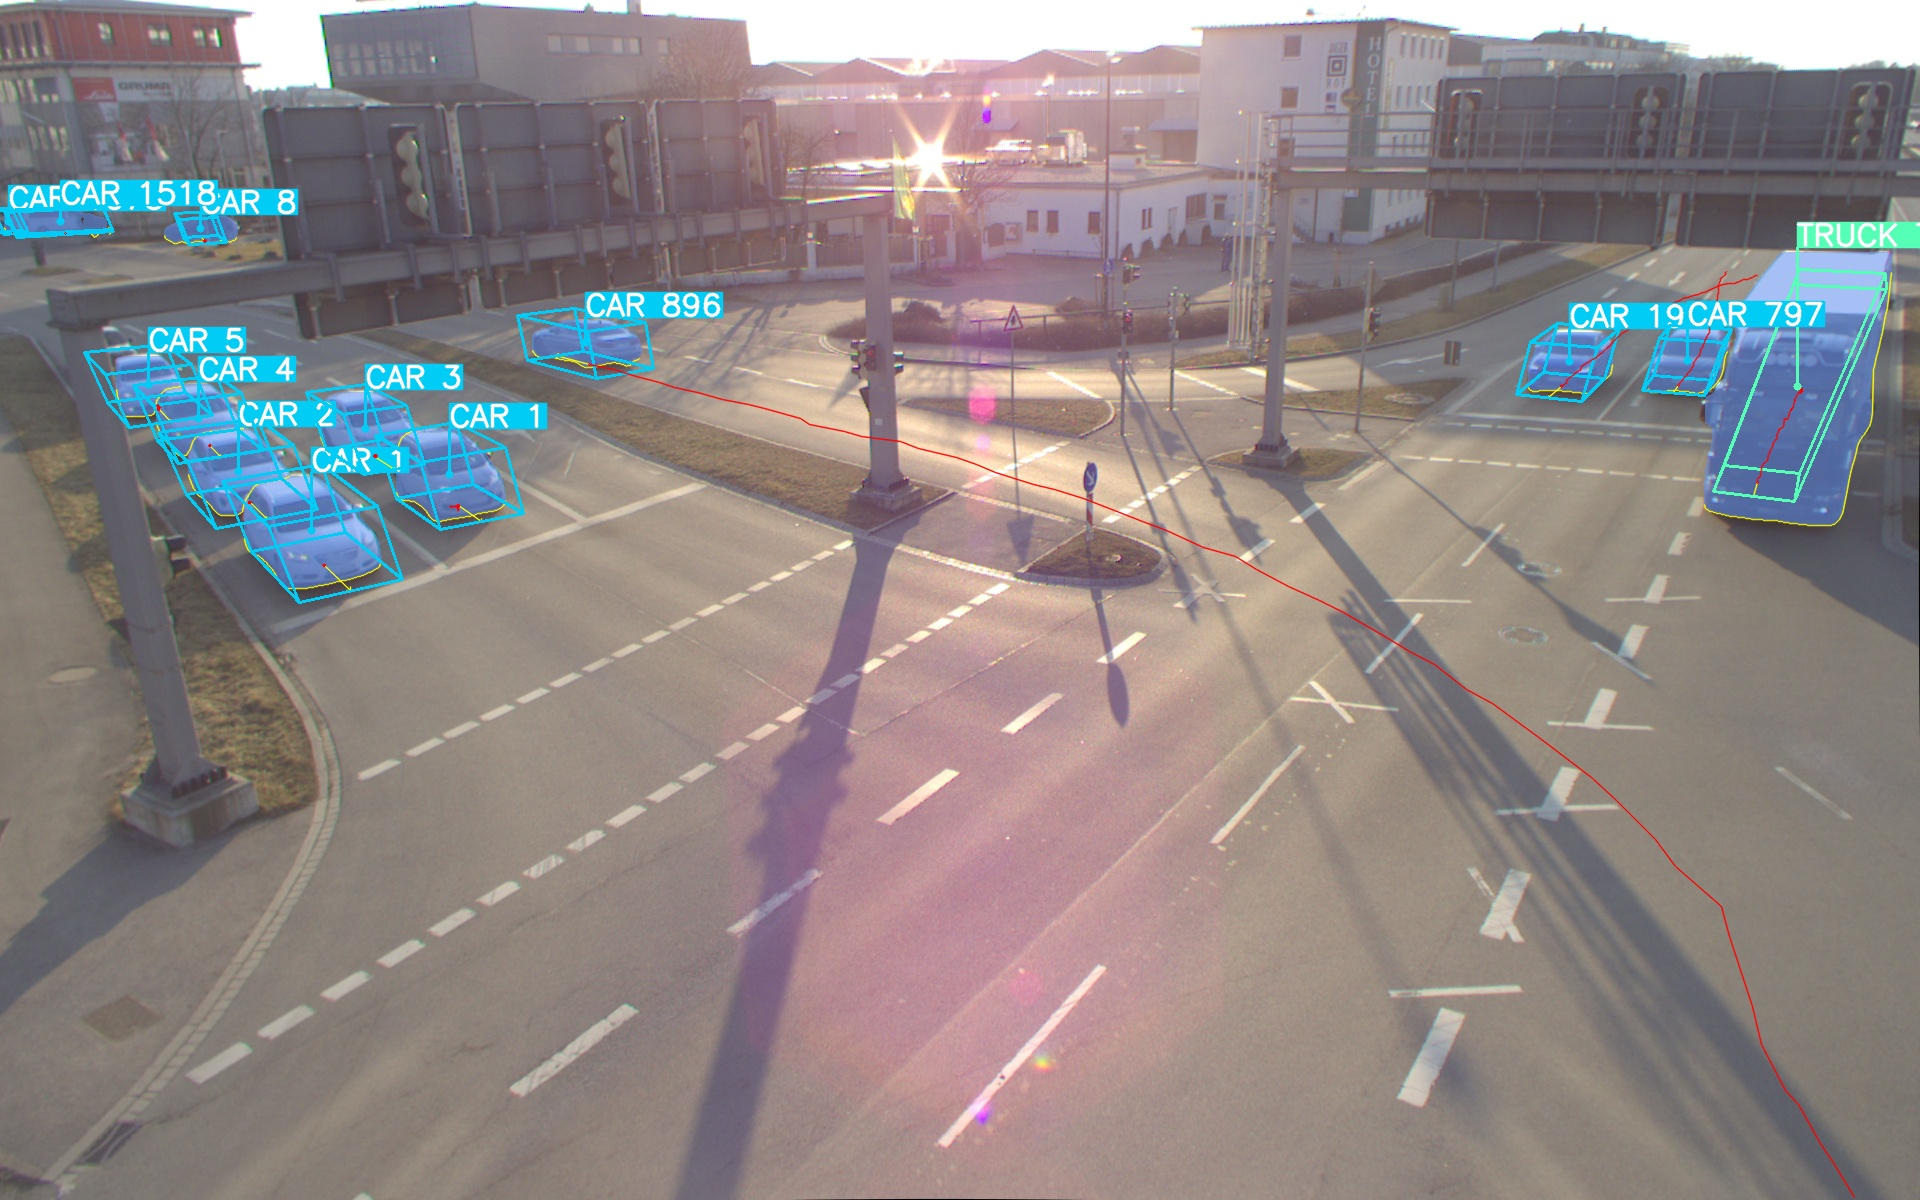
\includegraphics[width=0.499\linewidth]{
        figures/selection/1646667323.129810658.s110.camera.basler.south2.8mm}
    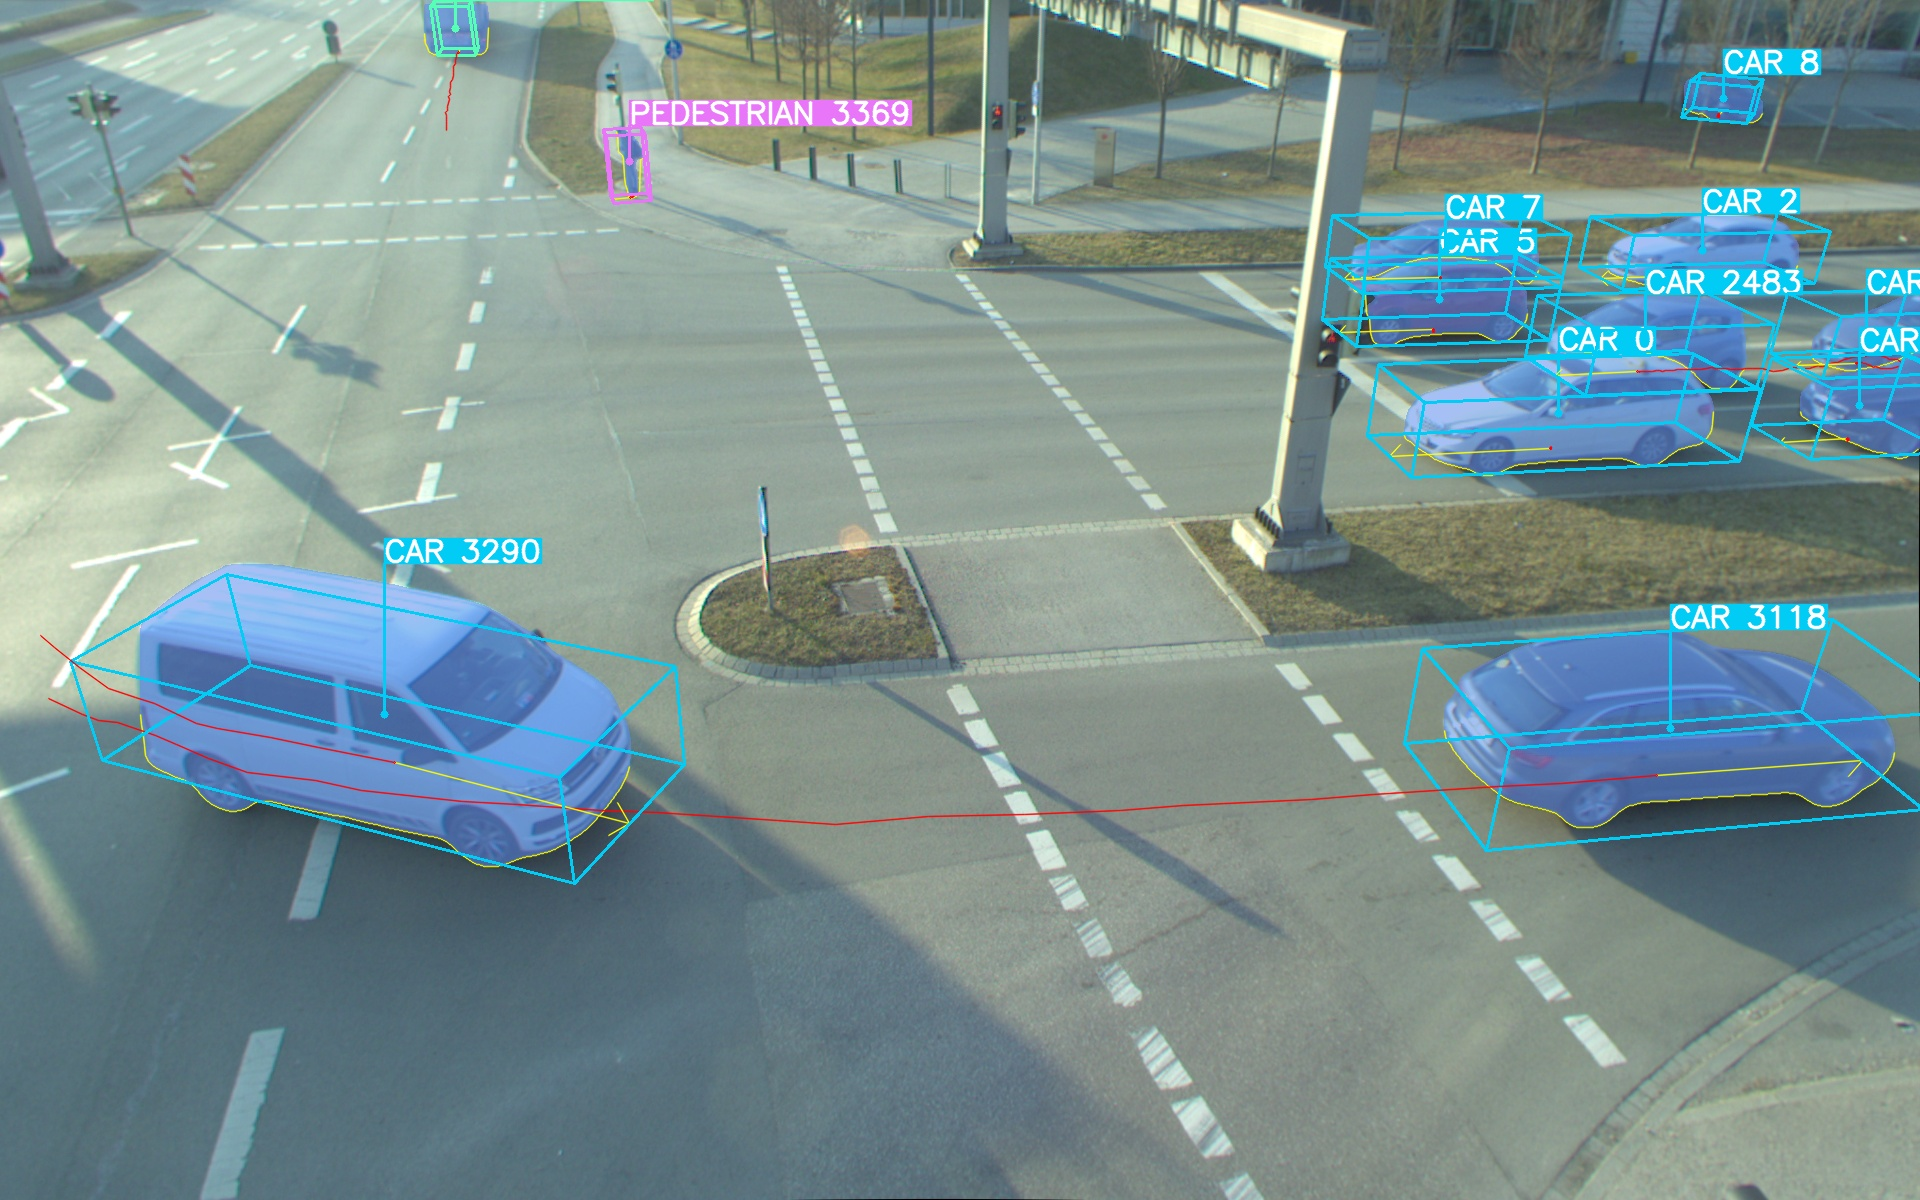
\includegraphics[width=0.499\linewidth]{
        figures/selection/1646667339.058779966.s110.camera.basler.south1.8mm} \\
    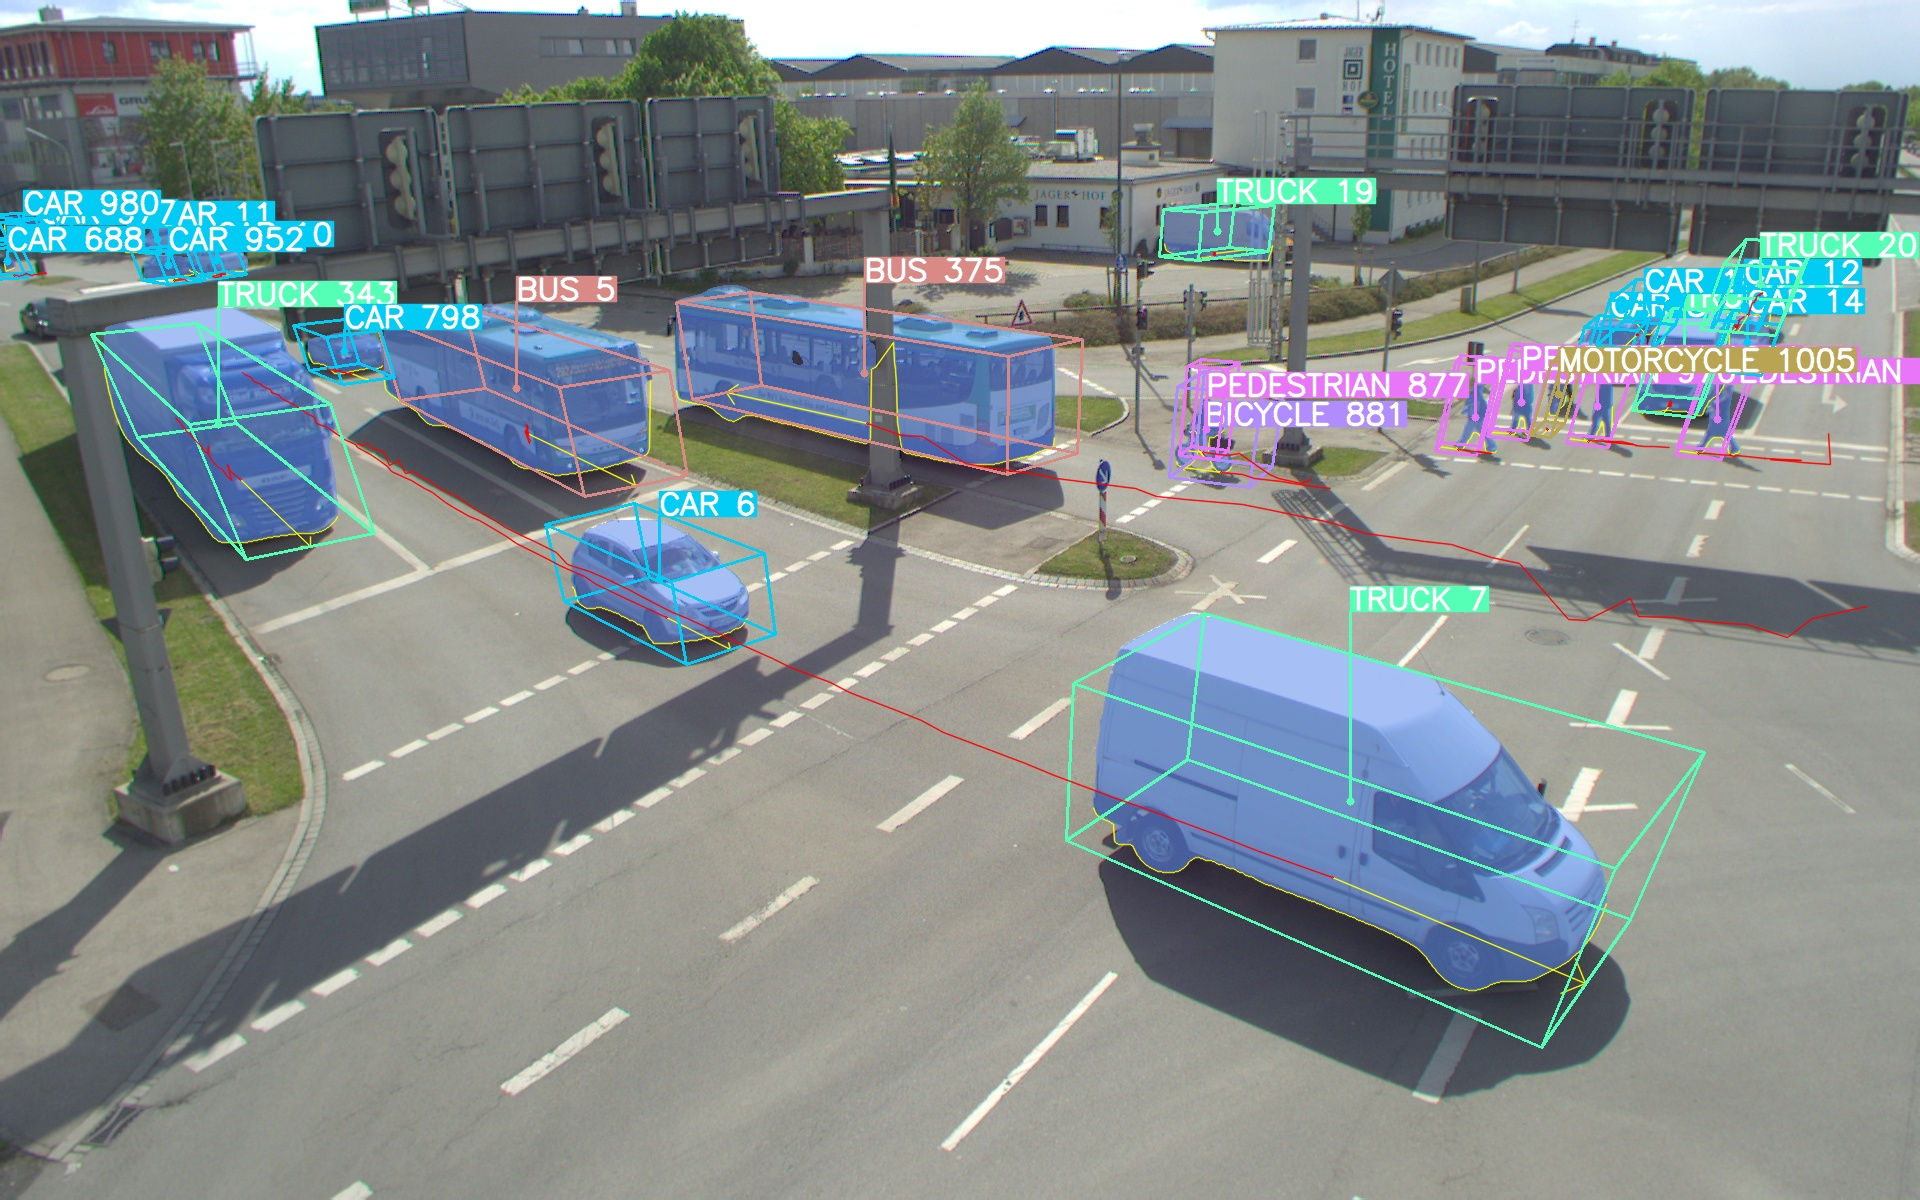
\includegraphics[width=0.499\linewidth]{
        figures/selection/1651673054.274505919.s110.camera.basler.south2.8mm}
    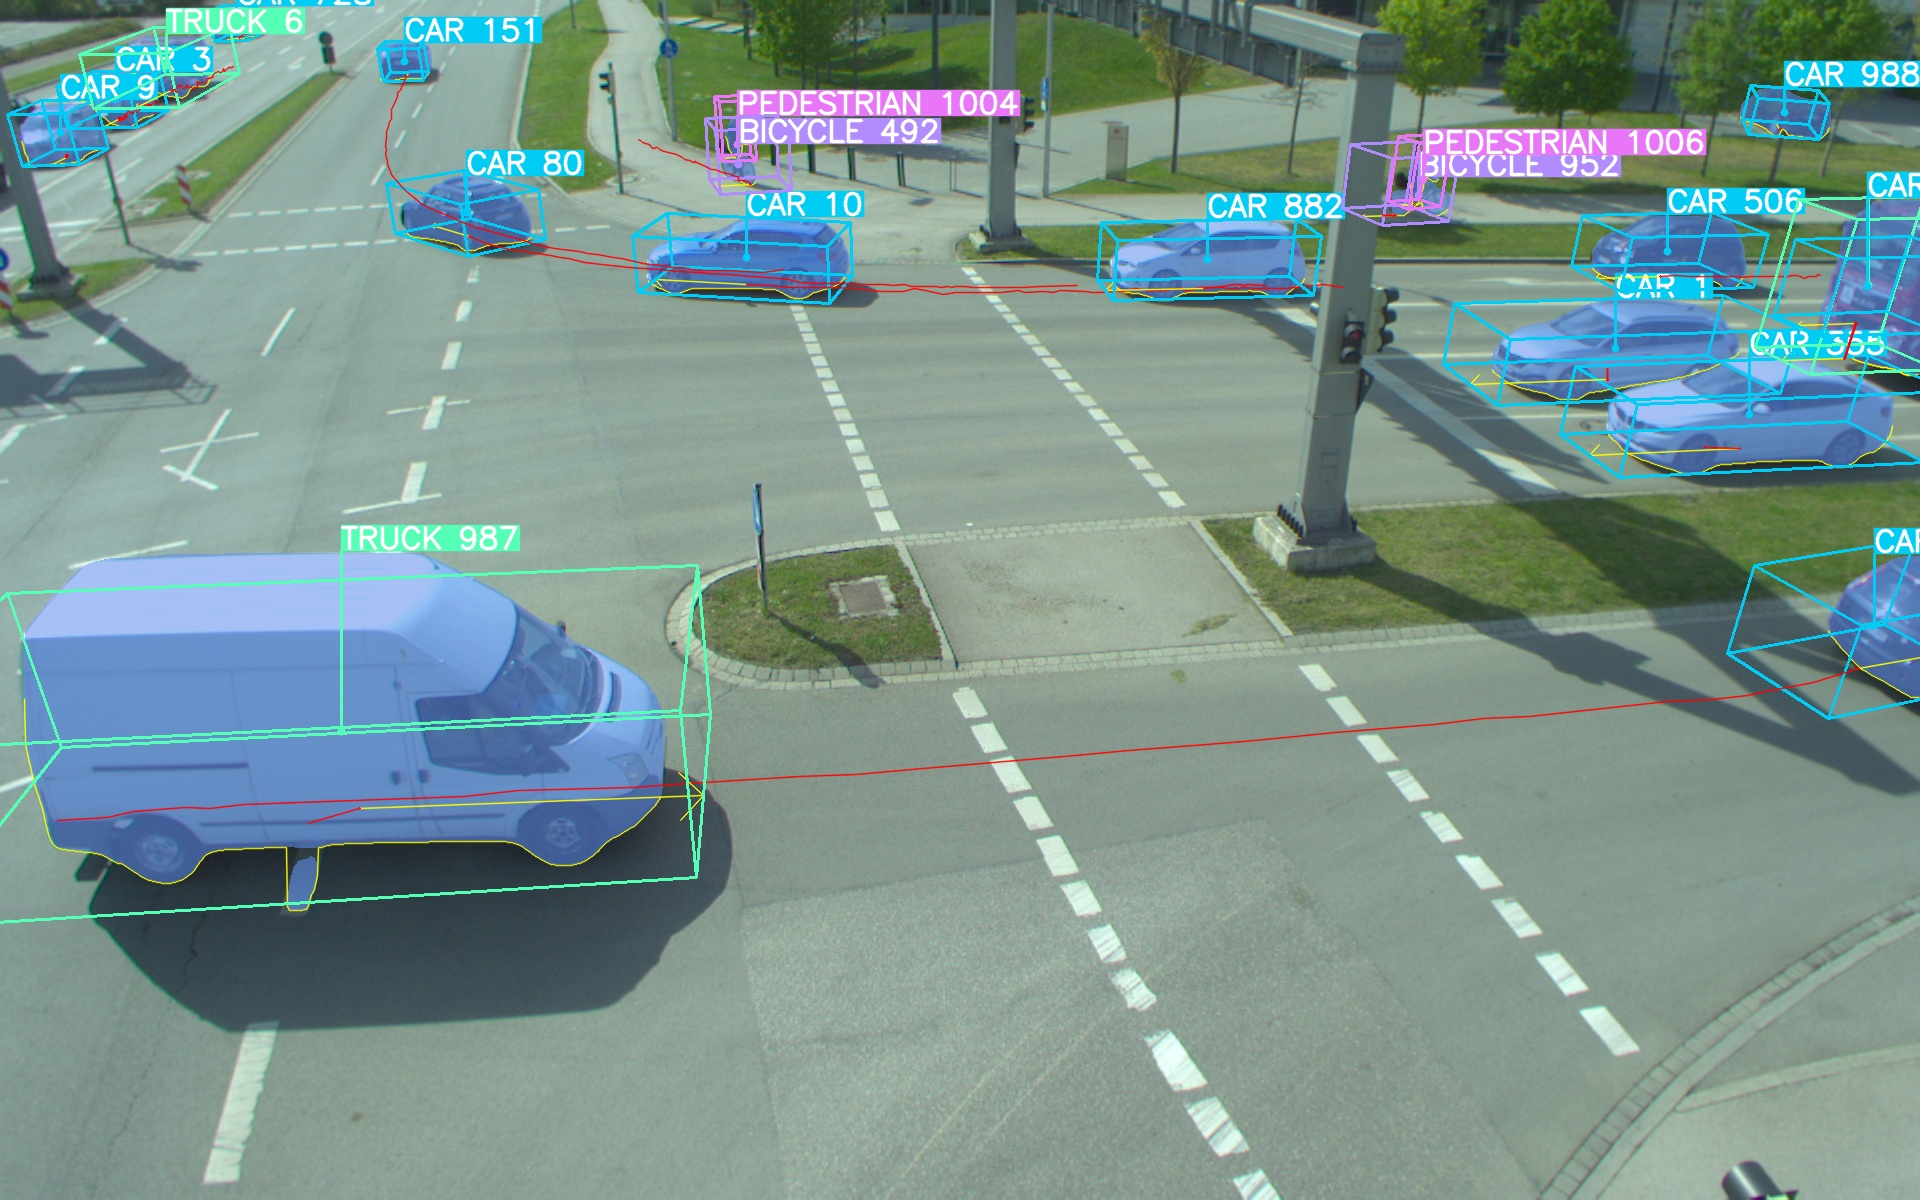
\includegraphics[width=0.499\linewidth]{
        figures/selection/1651673056.492970825.s110.camera.basler.south1.8mm}
    \caption{Hand-picked frames to showcase the qualitative performance of our implemented monocular 3D object detector at daytime.}
    \label{fig:qualitative-results-day}
\end{figure}

First off, Figure~\ref{fig:qualitative-results-day} shows representative frames with detection annotations, where the implemented system performs quite well.
The frames in the left column are from the South-2 camera, which has a greater detection range and wider field-of-view, as it is angled more towards towards the horizon.
The two frames for this camera show, that the implemented system can correctly detect the 3D shapes of many overlapping vehicles, which are oriented opposed or perpendicular to each other.
The top-left frame showcases the good performance of the screen-space \textit{SORT} tracker in particular, which tracks \texttt{CAR 896} throughout its whole left turn.
The bottom-left image shows the usefulness of the \textit{DBSCAN}-based bottom contour filter in the case of \texttt{BUS 375}.
The detection of this bus is split into two parts by the pole of the overhead gantry bridge.
This introduces a lot of noise into this detection's bottom contour, as highlighted in yellow.
However, the detected 3D bounding box is unaffected by this noise.
This frame also showcases the performance of our Vulnerable Road User (VRU) detection.
Both present pedestrians and bicycles in the image are correctly localized.

The frames in the right column are from the South-1 camera, which has a shorter detection range and narrower field-of-view, as it is angled more towards towards the ground.
Both images in the right column again show generally good vehicle tracking and orientation estimation capabilities.

\begin{figure}[htb]
    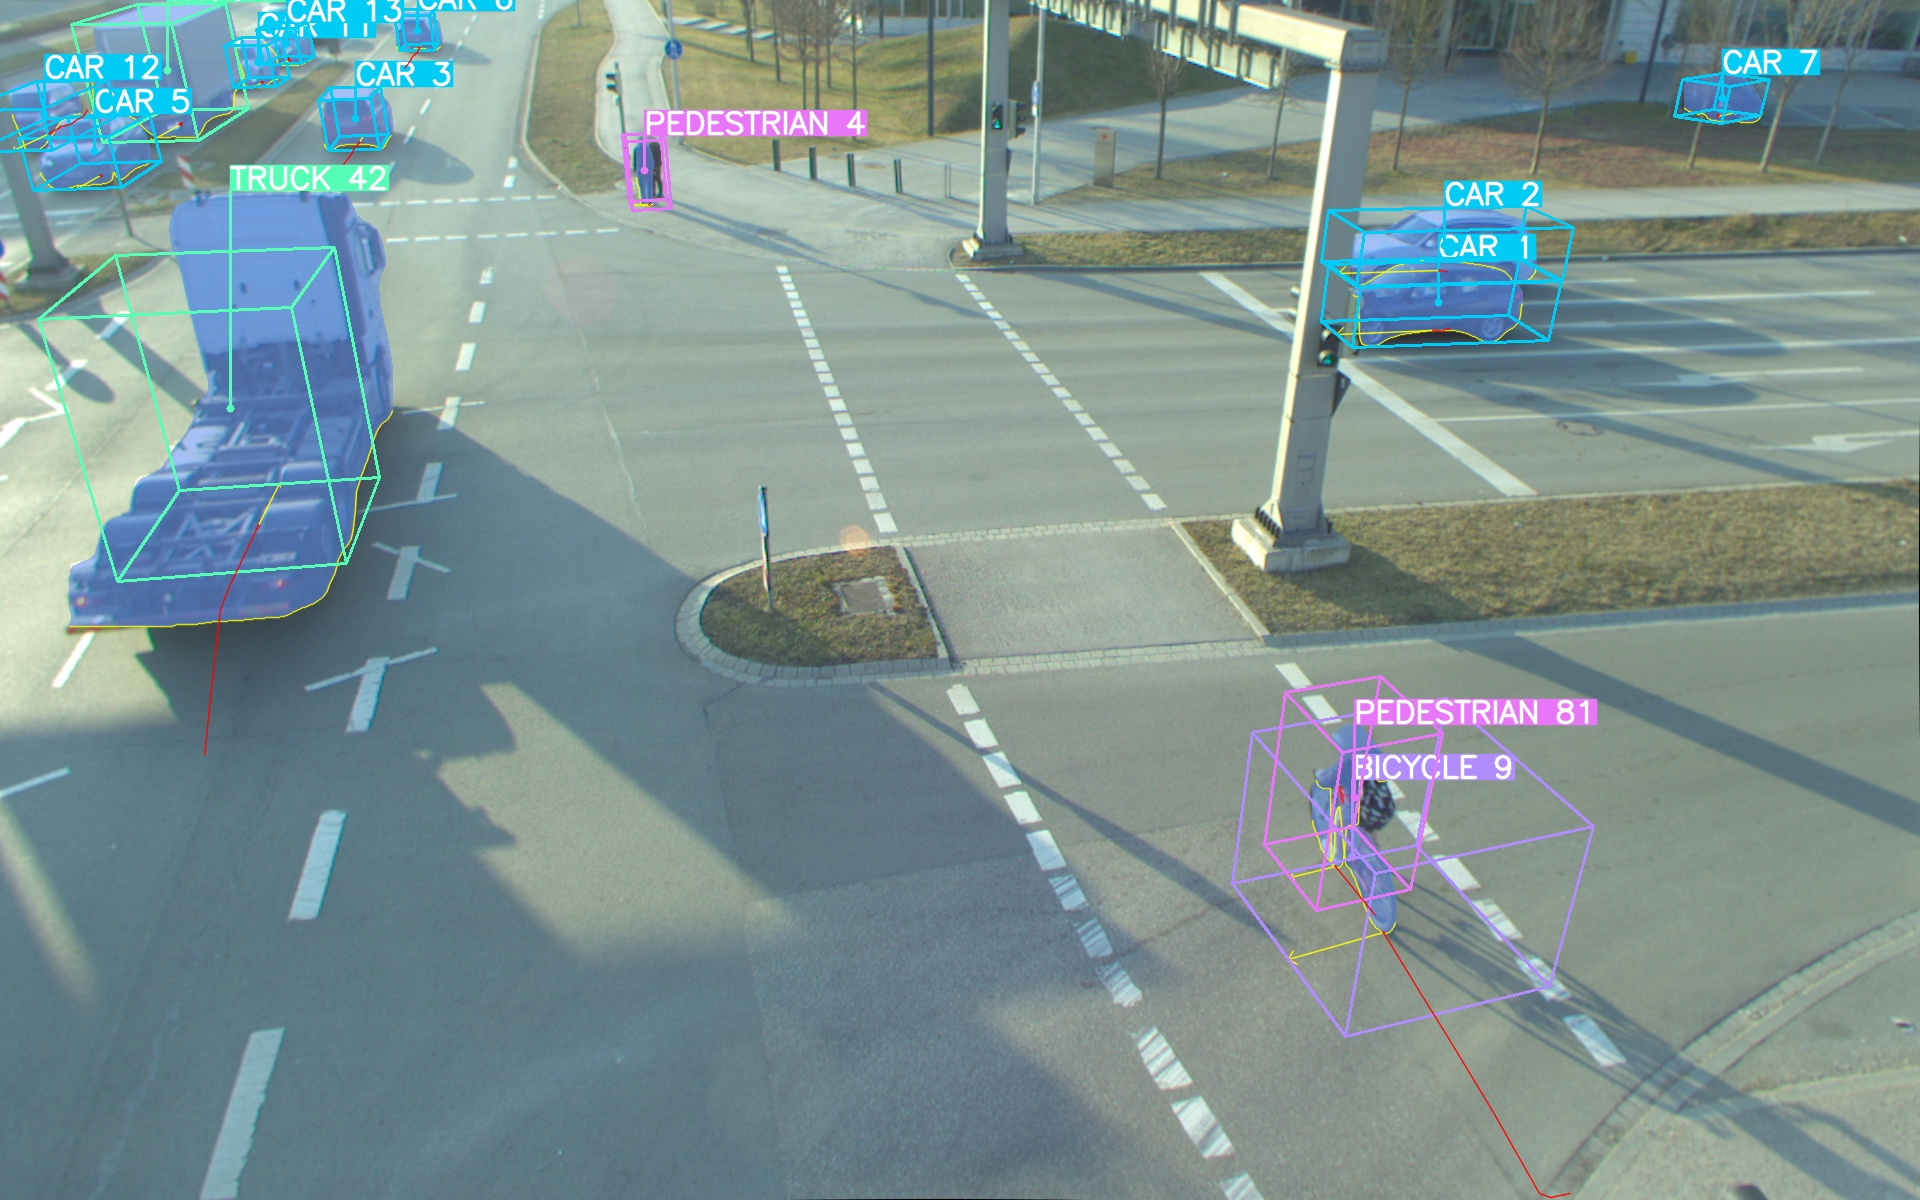
\includegraphics[width=0.499\linewidth]{
        figures/selection/1646667395.641065639.s110.camera.basler.south1.8mm}
    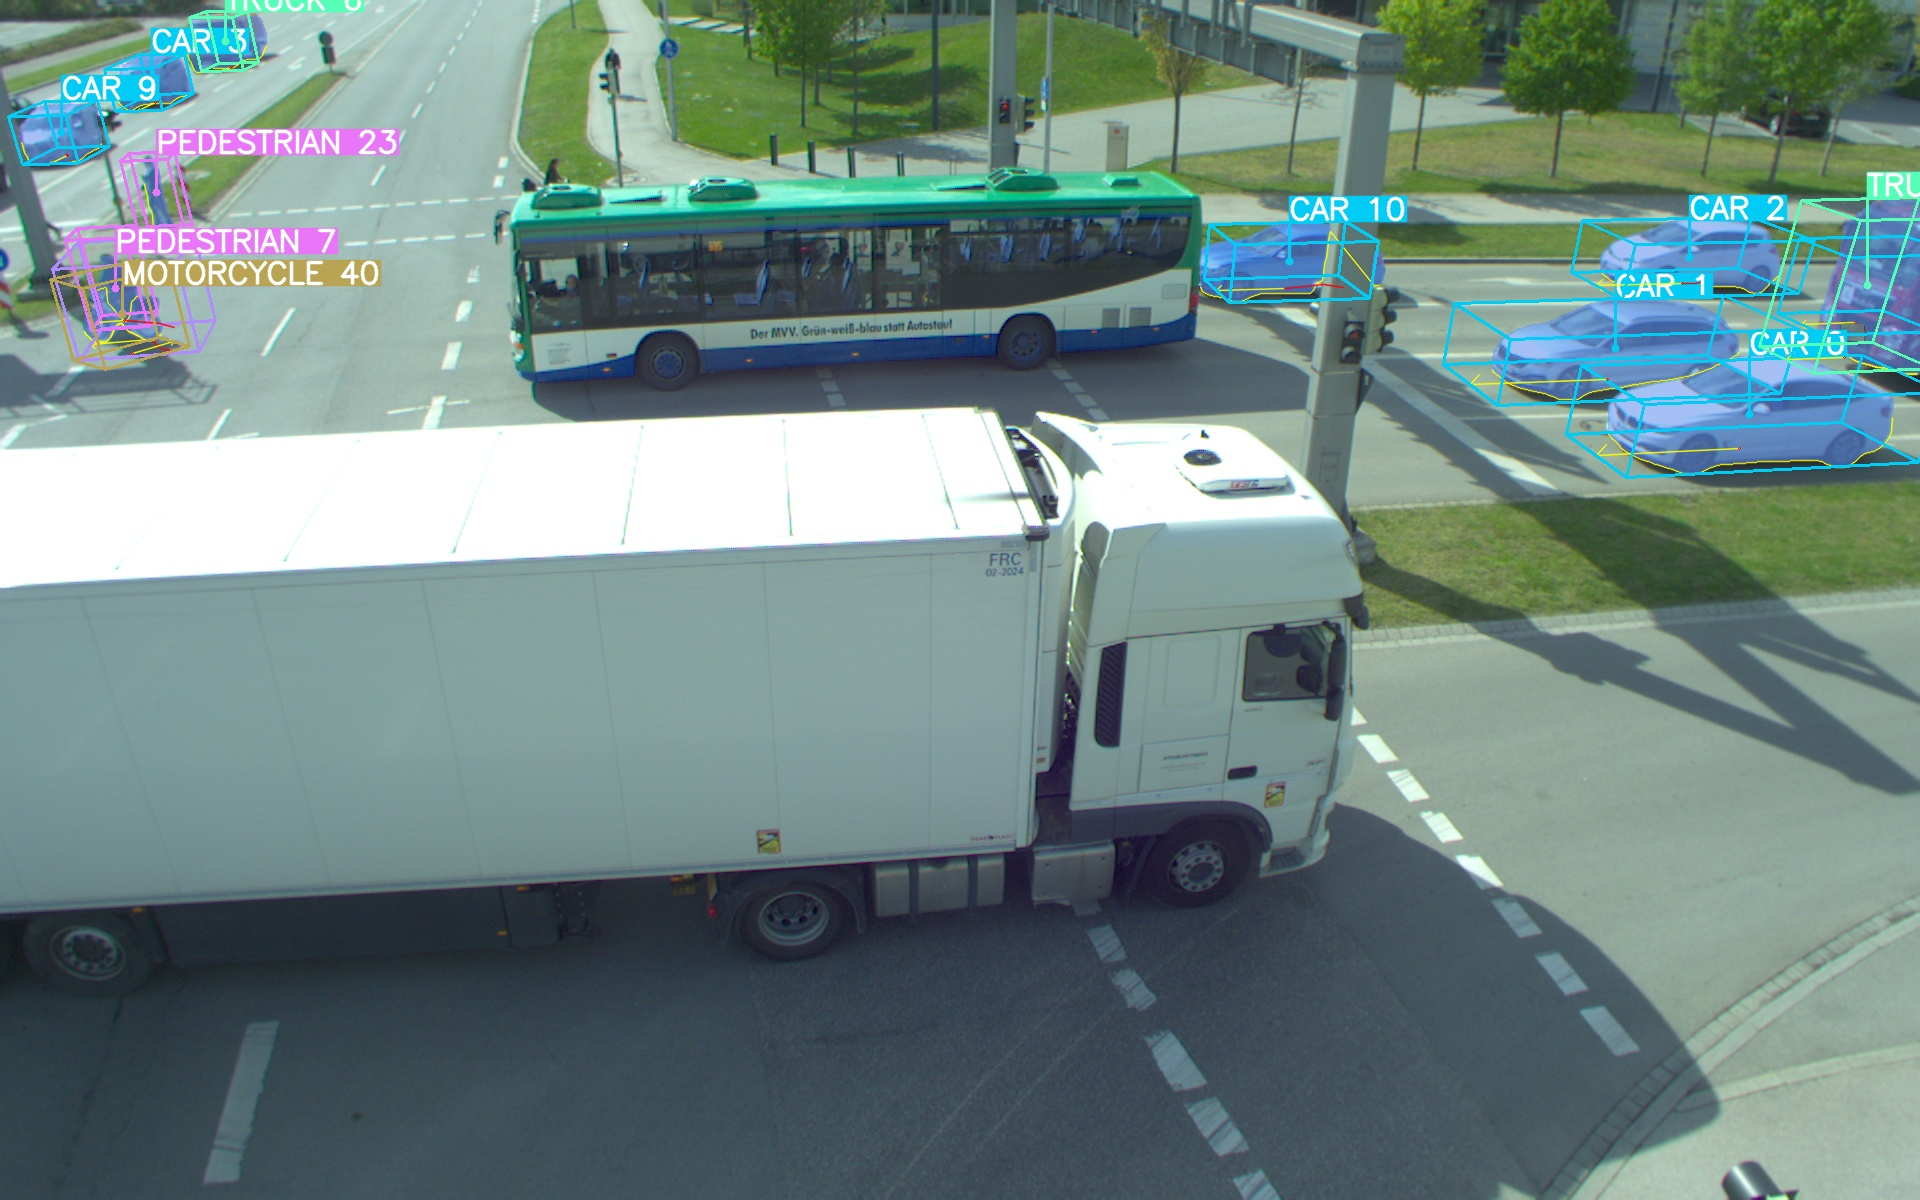
\includegraphics[width=0.499\linewidth]{
        figures/selection/1651673050.162472285.s110.camera.basler.south1.8mm}
    \caption{Selected frames to showcase particular problems of our implemented monocular 3D object detector.}
    \label{fig:qualitative-results-bad}
\end{figure}

Figure~\ref{fig:qualitative-results-bad} highlights particular weaknesses of the implemented monocular detector.
The image on the left highlights three problems.
First, the length estimation of \texttt{TRUCK 42} is bad, most likely due to over-eager bottom-countour filtering.
Second, only one of the two pedestrians is detected \textemdash \texttt{PEDESTRIAN 4} is standing next to another one.
Third, the system detects the rider of a bicycle as a separate entity, as in case of \texttt{BICYCLE 9} and \texttt{PEDESTRIAN 81}.
This points to a need for more fine-tuned non-maximum suppression (NMS) of 3D detections.
The image on the right shows a single problem: Our detector (more specifically the used \textit{Yolov7} instance segmentation model) frequently has problems with detecting the instance masks of large objects near the camera.
In this case, both the big white truck in front of the camera, and the bus which is a bit further away, are not detected.

\begin{figure}[htb]
    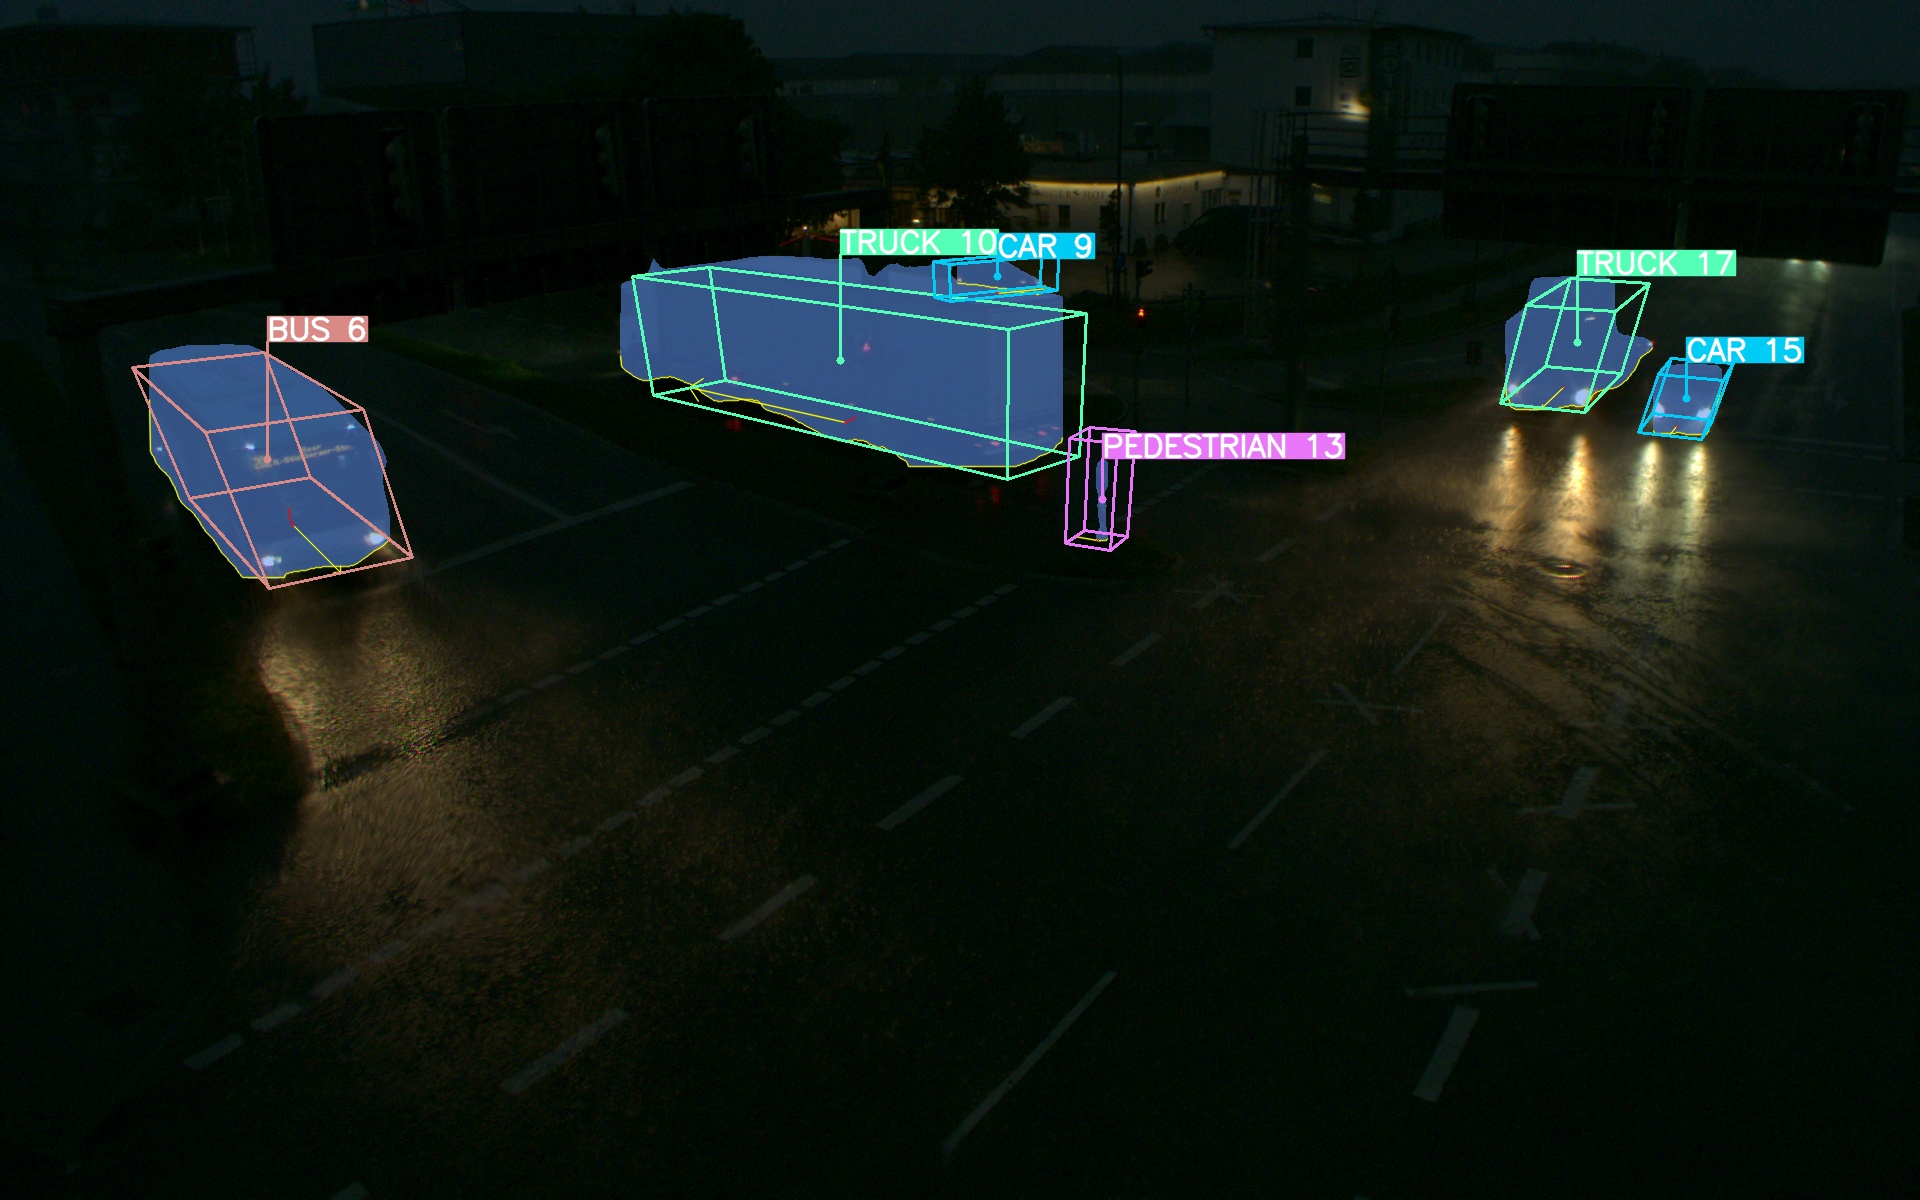
\includegraphics[width=0.499\linewidth]{
        figures/selection/1653330059.588901912.s110.camera.basler.south2.8mm}
    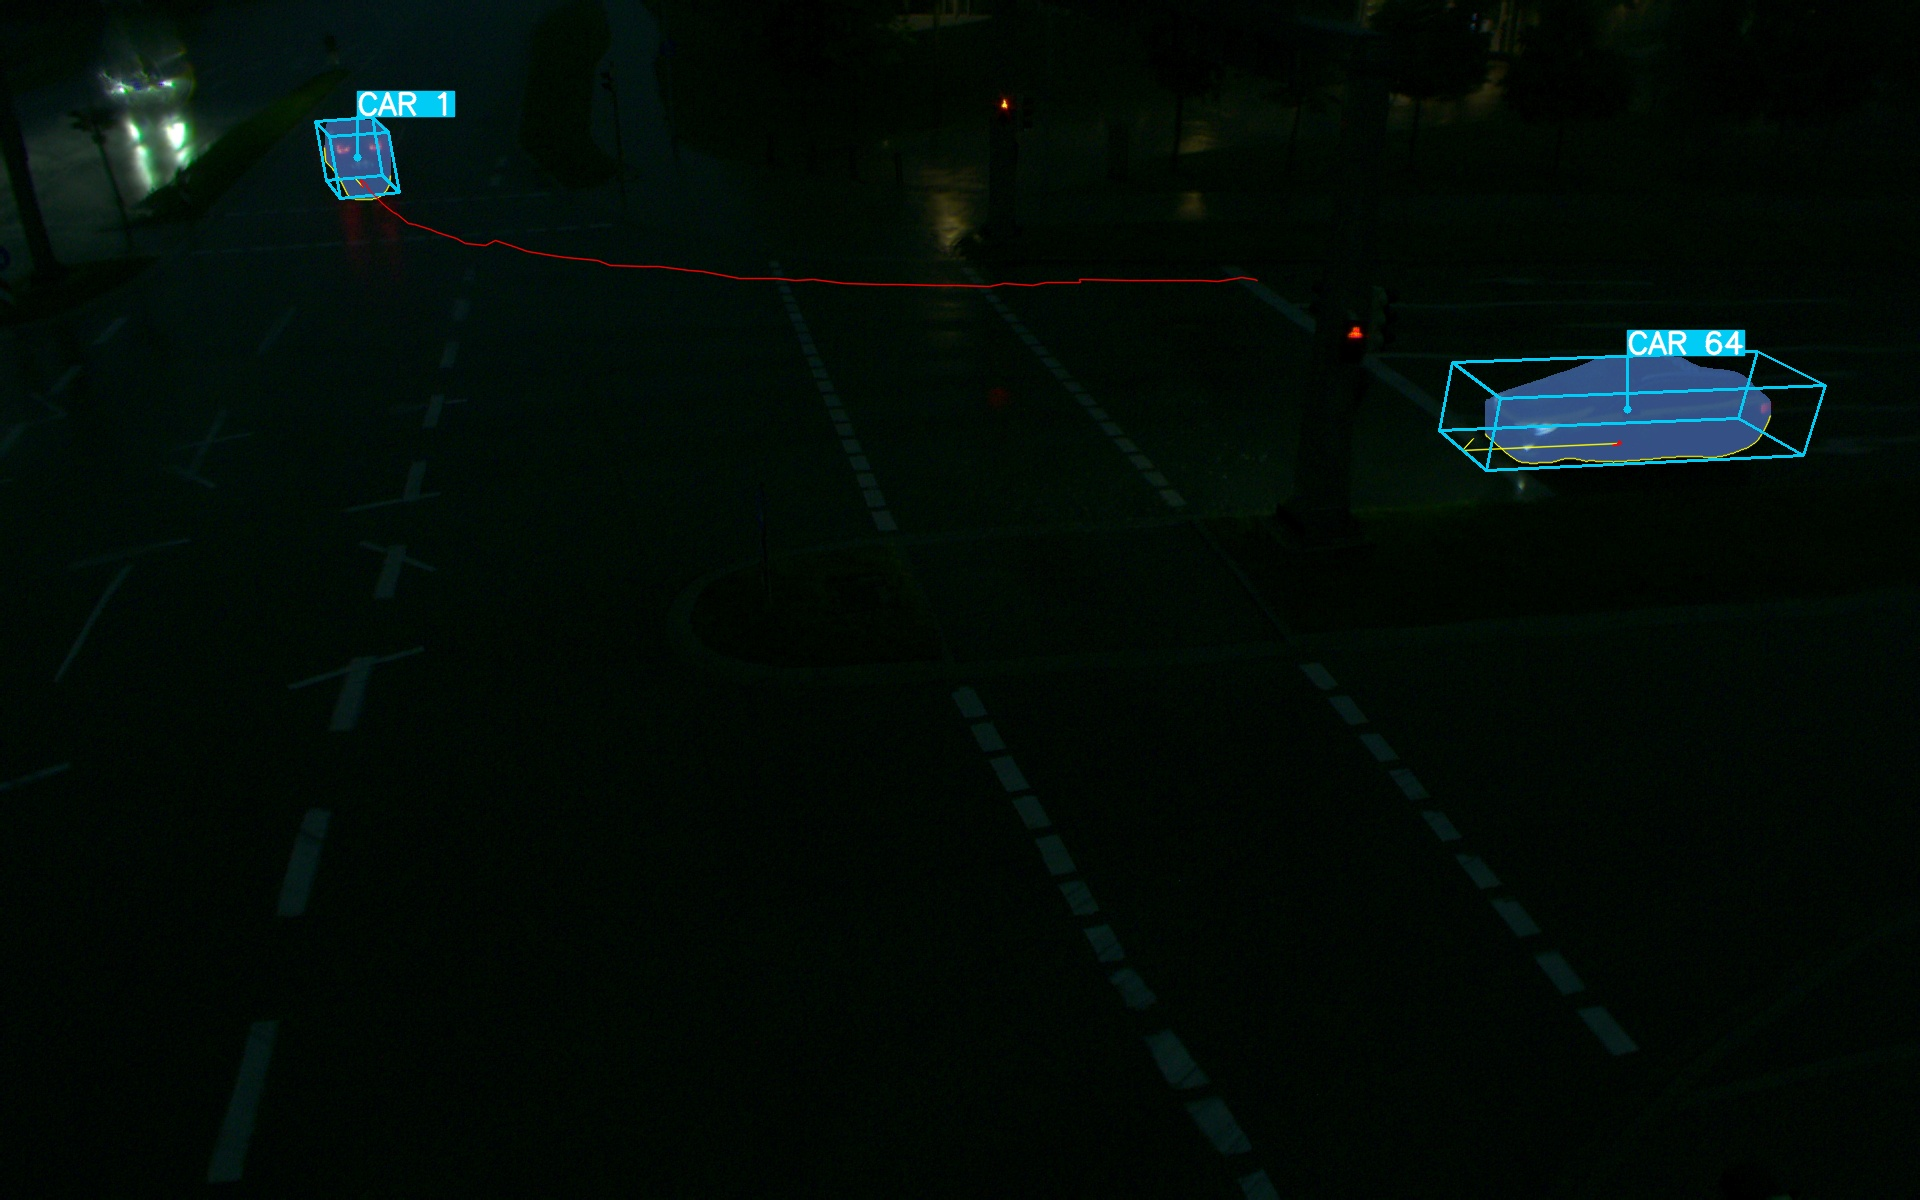
\includegraphics[width=0.499\linewidth]{
        figures/selection/1653330064.207615030.s110.camera.basler.south1.8mm}
    \caption{A selection of frames to showcase the qualitative performance of our implemented monocular 3D object detector at night.}
    \label{fig:qualitative-results-night}
\end{figure}

Finally, Figure~\ref{fig:qualitative-results-night} displays how the system performs at night.
Naturally, the detection performance of a system which is based on an RGB camera which operates in the human visible light spectrum will be worse at night, due to the reduced visibility.
However, the used \textit{Yolov7} instance segmentation model still works to some degree at night.
The predicted instance masks are generally noisier, and there more false positives (such as \texttt{PEDESTRIAN 13}) and false negatives (such as the truck on the top-left in the right image).

% ----------------------------------------------------

\section{Quantitative Evaluation Strategy}
\label{sec:quant}

For an objective understanding of the performance of our \textit{Mono3D} solution, we performed a thorough ablative quantitative evaluation.
For this purpose, we use the \textit{Providentia A9R1} dataset, as previously mentioned in the Introduction (see Chapter~\ref{sec:a9dataset}).
As stated, the dataset provides 3D lidar label annotations for two camera perspectives onto the urban \textit{S110} road intersections.
For each camera, four scenes of varying length (between 300 and 1200 frames) are available.
The combination of two camera perspectives and four scenes yields eight frame sequences on which we evaluate our detector.
For each frame sequence, the detector is run in different configurations to evaluate the effect of various design choices on the final performance.
The detector is configured along four major components:

\begin{enumerate}
    \item \textbf{Instance Segmentation}: In the first detector stage,\ We can employ the \textit{Yolact}~\cite{liu2021yolactedge} instance segmentation model (running on 550x550 input frames), or the \textit{YoloV7}~\cite{wang2022yolov7} detector in 640x640, 1280x180, or 1920x1920 px resolution mode.\ We respectively designate these modes as $I^{550}_\text{YOL}$, $I^{640}_\text{Yv7}$, $I^{1280}_\text{Yv7}$, and $I^{1920}_\text{Yv7}$.
    \item \textbf{Tracking}: This component concerns the usage of \textit{SORT tracking}~\cite{bewley2016simple} in our detector.\ We can apply tracking in $2D$ screen-space to assist the LSF algorithm, or in $3D$ space to stabilize vehicle position estimates, or both in $2D$ and $3D$, or not at all.\ We respectively designate these modes as $T_{2D}$, $T_{3D}$, $T^{2D}_{3D}$, and $T_0$.
    \item \textbf{HD-Map Usage}: In this aspect, we consider whether to use heading information from the HD-map as an early input to the LSF algorithm, as a late single-position lookup correction, or not at all.\ These modes are designated as $M_\text{LSF}$, $M_1$ and $M_0$.
    \item \textbf{Filtering}: Finally, we can switch two crucial filters on or off:\ The \textit{DBSCAN}~\cite{schubert2017dbscan} bottom contour point filter, and the output vehicle size filter.\ These modes will be symbolized as $F_\text{Cont}$, $F_\text{Size}$, $F_\text{Cont}^\text{Size}$, or $F_0$ (if no filter is used).
\end{enumerate}

In summary, each detector configuration is some combination of $I$, $T$, $M$ and $F$.\ For example, $\left[I^{640}_\text{Yv7}T^{2D}_{3D}M_\text{LSF}F_\text{Size}\right]$ would be the detector running with 640x640 px \textit{Yolov7} instance segmentation, both 2D and 3D tracking, L-Shape-Fitting Map Input, and vehicle size filtering (but no bottom-contour filtering).
The combinatorial expansion yields 192 possible detector configurations, which are executed on each of the 8 LIDAR-labeled camera frame sequences.
This results in 1536 prediction sequences.

Furthermore, we evaluate the impact which emerges from the sensor delay between the camera and the LIDAR sensor frames.
This delay is roughly 149ms on average.
This synchronization error is important, because we evaluate the 3D camera detections on labeled LIDAR sensor measurements.
These LIDAR labels will contain an inherent offset towards the camera detections due to the synchronization error.
We check whether the error can be reduced by estimating the spatial velocity of the LIDAR detections using \textit{SORT}, and then correcting the label position based on the velocity and the known synchronization error time delta.

We evaluate both the time-shifted and the original LIDAR labels with each prediction sequence.
We call these two label modes $L_0$ (original) and $L_{\uparrow}$ (shifted).
The label mode is appended to the detector configuration combination.
For each of the 3072 sequence-detector-label combinations and each road suer class, we calculate the following metrics:

\begin{enumerate}
    \item The average orientation error \textbf{(AOE)} ($=\text{TP}_0$).
    \item The average translation error \textbf{(ATE)} ($=\text{TP}_1$.
    \item The average length error \textbf{(ALE)} ($=\text{TP}_2$).
    \item The average width error \textbf{(AWE)} ($=\text{TP}_3$).
    \item The average height error \textbf{(AHE)} ($=\text{TP}_4$).
    \item The average precision at 10\% overlap \textbf{(AP@10)}.
    \item The average 3D intersection-over-union ($\mathbf{IoU}_{3D}$)
\end{enumerate}

In the following, the values for these metrics are presented in relation to particular detector and labeling configurations.
To judge the overall performance of a configuration, we aggregate these metrics into a single \enquote{Providentia Detection Score}, similar to the \textit{nuScenes Detection Score} (see Section~\ref{sec:evalmetrics}):

\[
    \text{Score} = \frac{1}{10} \left[5 * \text{mAP} + \sum^5_{k=1}(1-\text{min}(1, \text{mTP}_k))\right]
\]

The score is calculated for each configuration, by averaging the metrics of the configuration across all perspectives of all dataset scenes.
A chart of all calculated Scores is shown in Figure~\ref{fig:all-scores}.

% ----------------------------------------------------

\section{Overall Quantitative Results}
\label{sec:baseline}

\begin{figure}[htb]
    
        \begin{tikzpicture}
        \begin{axis}[
            clip=false,
            ybar,
            width=\textwidth,
            height=0.4\textwidth,
            bar width=0.1pt,
            ylabel={Score},
            ymin=10, ymax=50,
            xtick=\empty,
            xticklabels={},
            enlarge x limits={abs=1pt},
        ]        
        
            \addplot [draw=blue, fill=none] table [x=xpos, y=yvalue, col sep=comma]{charts/overall.tex.blue.dat};
            \draw[black, thin, -latex]([xshift=0.1pt]axis cs:1,10) -- ++(axis direction cs:0,-8)node[below, font=\tiny, anchor=north west, outer sep=0] {\textbf{Model}: $\left[I^{550}_\text{YOL}T^{2D}_{3D}M_1F_0L_{\uparrow}\right]$: $13.58$};
\draw[black, thin, -latex]([xshift=0.1pt]axis cs:12,10) -- ++(axis direction cs:0,-3)node[below, font=\tiny, anchor=north west, outer sep=0] {\textbf{Model}: $\left[I^{550}_\text{YOL}T_0M_0F_0L_0\right]$: $17.78$};
\draw[black, thin, -latex]([xshift=0.1pt]axis cs:384,10) -- ++(axis direction cs:0,-3)node[below, font=\tiny, anchor=north east, outer sep=0] {\textbf{Model}: $\left[I^{1920}_\text{Yv7}T_{2D}M_\text{LSF}F_\text{Cont}^\text{Size}L_{\uparrow}\right]$: $40.17$};

        \end{axis}
        \end{tikzpicture}
        
    \caption{Overview for the Score values of all possible 384 detector configuration-label combinations, with arrows pointing out the best, baseline, and worst combination.}
    \label{fig:all-scores}
\end{figure}

In order to establish the veracity of our score metric, we plotted the score values for all possible 384 detector configuration-label combinations into a single chart.
This plot is shown in Figure~\ref{fig:all-scores}.
In this plot, the Scores of the worst-performing- ($\left[I^{550}_\text{YOL}T^{2D}_{3D}M_1F_0L_{\uparrow}\right]$), baseline- ( $\left[I^{550}_\text{YOL}T_0M_0F_0L_0\right]$), and best-performing ($\left[I^{1920}_\text{Yv7}T_{2D}M_\text{LSF}F_\text{Cont}^\text{Size}L_{\uparrow}\right]$) model-configurations are also highlighted.
The baseline model works with pure L-Shape-Fitting that does not use any HD-map, tracking, or bottom-contour/size filtering augmentations.
Table~\ref{tbl:baseline} shows the performance of this model in greater detail.
Of particular interest is the fairly large AOE of $45.44\degree$.
This means, that the predicted orientation of bounding boxes in this model is essentially completely disconnected from the ground truth.
Picking a random orientation would yield the same result.

\begin{table*}[htbp]
    
        \centering
        \scalebox{0.91}{
        \begin{tabular}{|l|rrrrrr|rrr|}
\hline & \multicolumn{6}{l|}{\textbf{Model}: $\left[I^{550}_\text{YOL}T_0M_0F_0L_0\right]$} & \multicolumn{3}{l|}{\textbf{PDS}: $15.31\%$} \rule{0pt}{1.4em} \\[0.2em] 

            \hline
            \hline
            \textbf{Class} & \textbf{AOE} & \textbf{ATE} & \textbf{AWE} & \textbf{ALE} & \textbf{AHE} & $\mathbf{IoU}_{3D}$ & \textbf{Precision} & \textbf{Recall} & \textbf{AP}{@}10 \\ 

            \hline
            Car & $57.39\degree$ & $1.10\nobreak\hspace{{.16667em plus .08333em}}m$ & $0.49\nobreak\hspace{{.16667em plus .08333em}}m$ & $1.03\nobreak\hspace{{.16667em plus .08333em}}m$ & $0.69\nobreak\hspace{{.16667em plus .08333em}}m$ & $21.80\%$ & $47.60\%$ & $40.57\%$ & $46.85\%$ \\ 
Truck & $34.61\degree$ & $2.17\nobreak\hspace{{.16667em plus .08333em}}m$ & $0.77\nobreak\hspace{{.16667em plus .08333em}}m$ & $4.15\nobreak\hspace{{.16667em plus .08333em}}m$ & $1.31\nobreak\hspace{{.16667em plus .08333em}}m$ & $20.31\%$ & $3.55\%$ & $1.67\%$ & $2.86\%$ \\ 
Motorcycle & $71.98\degree$ & $0.63\nobreak\hspace{{.16667em plus .08333em}}m$ & $0.76\nobreak\hspace{{.16667em plus .08333em}}m$ & $1.31\nobreak\hspace{{.16667em plus .08333em}}m$ & $0.13\nobreak\hspace{{.16667em plus .08333em}}m$ & $14.72\%$ & $31.14\%$ & $22.98\%$ & $30.68\%$ \\ 
Bus & $44.76\degree$ & $1.85\nobreak\hspace{{.16667em plus .08333em}}m$ & $1.47\nobreak\hspace{{.16667em plus .08333em}}m$ & $3.07\nobreak\hspace{{.16667em plus .08333em}}m$ & $1.55\nobreak\hspace{{.16667em plus .08333em}}m$ & $22.47\%$ & $17.47\%$ & $10.51\%$ & $16.19\%$ \\ 
Pedestrian & \textemdash & $0.38\nobreak\hspace{{.16667em plus .08333em}}m$ & $0.25\nobreak\hspace{{.16667em plus .08333em}}m$ & $0.18\nobreak\hspace{{.16667em plus .08333em}}m$ & $0.07\nobreak\hspace{{.16667em plus .08333em}}m$ & $21.62\%$ & $0.88\%$ & $0.10\%$ & $0.65\%$ \\ 
Bicycle & \textemdash & $0.34\nobreak\hspace{{.16667em plus .08333em}}m$ & $0.65\nobreak\hspace{{.16667em plus .08333em}}m$ & $0.46\nobreak\hspace{{.16667em plus .08333em}}m$ & $0.10\nobreak\hspace{{.16667em plus .08333em}}m$ & $20.46\%$ & $0.92\%$ & $0.17\%$ & $0.67\%$ \\ 

\hline
\textbf{Mean} & $\mathbf{52.19\degree}$ & $\mathbf{1.08\nobreak\hspace{{.16667em plus .08333em}}m}$ & $\mathbf{0.73\nobreak\hspace{{.16667em plus .08333em}}m}$ & $\mathbf{1.70\nobreak\hspace{{.16667em plus .08333em}}m}$ & $\mathbf{0.64\nobreak\hspace{{.16667em plus .08333em}}m}$ & $\mathbf{20.23\%}$ & $\mathbf{16.93\%}$ & $\mathbf{12.67\%}$ & $\mathbf{16.31\%}$ \\ 

            \hline
            
        \end{tabular}
        }
    \caption{Baseline model results.}
    \label{tbl:baseline}
\end{table*}

This stands in contrast to the performance metrics for the best-performing model, which are shown in Table~\ref{tbl:best}.
In the following sections, we will discuss in detail how specific model configurations improve (or worsen) specific metrics for different road user classes.

\begin{table*}[htbp]
    
        \centering
        \scalebox{0.91}{
        \begin{tabular}{|l|rrrrrr|rrr|}
\hline & \multicolumn{6}{l|}{\textbf{Model}: $\left[I^{1920}_\text{Yv7}T_{2D}M_\text{LSF}F_\text{Cont}^\text{Size}L_{\uparrow}\right]$} & \multicolumn{3}{l|}{\textbf{Score}: $40.29\%$ $({\scriptstyle\color{TUMGreen}+24.98\%})$} \rule{0pt}{1.4em} \\[0.2em] 

            \hline
            \hline
            \textbf{Class} & \textbf{AOE} & \textbf{ATE} & \textbf{AWE} & \textbf{ALE} & \textbf{AHE} & $\mathbf{IoU}_{3D}$ & \textbf{Precision} & \textbf{Recall} & \textbf{AP}{@}10 \\ 

            \hline
            Car & $3.13\degree$ & $0.85m$ & $0.25m$ & $0.89m$ & $0.35m$ & $39.19\%$ & $72.76\%$ & $73.19\%$ & $72.26\%$ \\ 
Truck & $4.16\degree$ & $1.69m$ & $0.62m$ & $2.52m$ & $0.58m$ & $17.67\%$ & $23.47\%$ & $28.83\%$ & $22.84\%$ \\ 
Motorcycle & $3.85\degree$ & $0.78m$ & $0.31m$ & $0.63m$ & $0.14m$ & $26.91\%$ & $34.22\%$ & $30.43\%$ & $33.88\%$ \\ 
Bus & $10.35\degree$ & $1.15m$ & $0.55m$ & $2.93m$ & $1.08m$ & $33.55\%$ & $51.71\%$ & $35.50\%$ & $50.74\%$ \\ 
Pedestrian & \textemdash & $0.38m$ & $0.28m$ & $0.20m$ & $0.07m$ & $32.26\%$ & $20.84\%$ & $13.55\%$ & $20.45\%$ \\ 
Bicycle & \textemdash & $0.56m$ & $1.22m$ & $0.69m$ & $0.08m$ & $21.99\%$ & $33.75\%$ & $35.33\%$ & $33.49\%$ \\ 

\hline
\textbf{Mean} & $\mathbf{5.37\degree}$ & $\mathbf{0.90m}$ & $\mathbf{0.54m}$ & $\mathbf{1.31m}$ & $\mathbf{0.38m}$ & $\mathbf{28.59\%}$ & $\mathbf{39.46\%}$ & $\mathbf{36.14\%}$ & $\mathbf{38.94\%}$ \\ 
$\Delta$ {Baseline} & ${\scriptstyle\color{TUMGreen}-46.81\degree}$ & ${\scriptstyle\color{TUMGreen}-0.18m}$ & ${\scriptstyle\color{TUMGreen}-0.19m}$ & ${\scriptstyle\color{TUMGreen}-0.39m}$ & ${\scriptstyle\color{TUMGreen}-0.26m}$ & ${\scriptstyle\color{TUMGreen}+8.36\%}$ & ${\scriptstyle\color{TUMGreen}+22.53\%}$ & ${\scriptstyle\color{TUMGreen}+23.47\%}$ & ${\scriptstyle\color{TUMGreen}+22.63\%}$ \\ 

            \hline
            
        \end{tabular}
        }
    \caption{Best model results, with improvements towards the baseline highlighted in green for each metric.}
    \label{tbl:best}
\end{table*}

% ----------------------------------------------------

\section{Impact of Late HD Map Lookup}
\label{sec:impactlatemap}

Impact of Late HD Map Lookup

Showcase qualitative evidence to support conclusions

\newpage

% ----------------------------------------------------

\section{Impact of YOLOv7 and Image Resolution}
\label{sec:impactyolov7}

Impact of YOLOv7

Showcase qualitative evidence to support conclusions

\newpage

% ----------------------------------------------------

\section{Impact of Bottom Contour Filtering}
\label{sec:impactcontourfiltering}

Impact of Bottom Contour Filtering

Showcase qualitative evidence to support conclusions

\newpage

% ----------------------------------------------------

\section{Impact of Dimension Filtering}
\label{sec:impactsizefiltering}

Impact of Category-based Dimension Clamping

Showcase qualitative evidence to support conclusions

\newpage

% ----------------------------------------------------

\section{Impact of HD-Map for L-Shape-Fitting}
\label{sec:impactearlymap}

Impact of Early HD Map Lookup

Showcase qualitative evidence to support conclusions

\newpage

% ----------------------------------------------------

\section{Impact of Tracking for L-Shape-Fitting}
\label{sec:impacthistplausibility}

Impact of Historical Plausibility

Showcase qualitative evidence to support conclusions

\newpage

% ----------------------------------------------------

\section{Impact of 3D Tracking}
\label{sec:impacttracking}

Impact of 3D Tracking

\newpage

% ----------------------------------------------------

\section{Impact of LIDAR Label Shifting}
\label{sec:impactlabelshifting}

Impact of LIDAR Label Shifting

Showcase qualitative evidence to support conclusions

\newpage

% ----------------------------------------------------

\section{Impact of Weather/Daytime Conditions}
\label{sec:weather}

Impact of Weather conditions

Showcase qualitative evidence to support conclusions

\newpage

% ----------------------------------------------------

\section{Performance}
\label{sec:performance}

Performance

% ----------------------------------------------------

\section{Summary}
\label{sec:summary}

Summarize evaluation results

% ----------------------------------------------------
